\section{Introduction}
\subsection{Motivation}
 
The initial brief for the project was simple. It was in the form of a challenge: Can you do this or better? It referred to a video of anonymous hands using the iSeeNotes app to take a picture of Mozart�s Rondo Alla Turca which was then played before our eyes.

\begin{figure}[ht!]
    \centering
    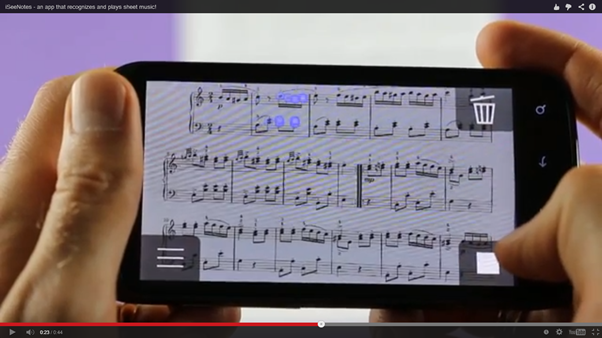
\includegraphics[width=120mm]{./assets/iseenotes.png}
    \caption{iSeeNotes Demo}
    \label{iseenotes}
\end{figure}
 
To us the challenge was irresistible. The opportunity to work on something that was very practically applicable was appealing. The applications of such software can be demonstrated in some of the early user stories we came up with:

\begin{itemize}
  \item A singer is learning to sight read music. He can take a picture of the sheet music with the app and it will play the notes so they can learn them.
  \item A saxophonist wants to play a duet but finds herself alone, she takes a picture of the accompaniment with the app and it plays the piano part.
  \item A child learning to read music, uses the app to bring the sheet music to life
  \item A Trumpet player needs to transpose a piece in to Bb from concert key, and our app allows them to shift the pitch in real time, without having to laboriously input each note into a music notation program by hand.
  \item A musician has a printed copy of some music, but wants to archive it or share it. Our app could allow them to do this, and actually enhance the original quality of the sheet music.
\end{itemize}
\subsection{Objectives}
We wanted to be able to reliably interpret sheet music from a photograph taken on a mobile device. We knew from the start that we weren�t going to be able to compete with existing desktop systems; their superior processing power and high quality scanned images make that an impossible task for a mobile device to compete with. What we therefore aimed to do is create a mobile OMR system that fulfills the following criteria:

\begin{itemize}
  \item Lighting tolerant: Our application should be able to scan images even where uniform lighting isn�t possible
  \item Distortion tolerant: Our application should be able to correct unavoidable perspective distortion found in even the highest quality photos.
  \item Speed: Despite the limited processing power of the devices we were working with, our application should be able to process the sheet music in a reasonable time, less than 30 seconds.
\end{itemize}

Our first objective was to get the app to be able to recognise and play a simple C major scale, followed by the nursery rhyme Baa Baa Black sheep. As we move on we wanted Sight Reader to recognise more complex music culminating in Fantasie Impromptu by Chopin. We then wanted the app to be able to save an output midi for the pieces.

\subsection{Contributions}
We have created an app that is able to:

\begin{itemize}
  \item interact with a device camera and take and save a picture
  \item process that image using Computer Vision techniques to recognise music represented on it including: staves, clefs, time signatures, crotchets, accidentals (flats, sharps and naturals), beams, half notes, quavers, quaver rests, dots, quavers
  \item concatenate music from multiple images
  \item produce and save a midi file of the music recognised
  \item allow playback of previously process music
\end{itemize}

All of this can be done portably using an android device. We have also managed to keep the response times within reasonable bounds.
